\chapter{Lịch sử nhiệt, tán xạ lần cuối và súp nguyên thủy}

\lectureoverview{Lịch sử giãn nở của vũ trụ cũng là một lịch sử nhiệt. Ta bắt đầu bằng cách định nghĩa nhiệt độ thông qua cân bằng, và định nghĩa cân bằng thông qua tán xạ. Một khí photon có được phổ Planck chừng nào các điện tích tự do còn giữ cho nó ở trạng thái cân bằng nhiệt; khi electron liên kết với proton, bức xạ tách rời nhưng vẫn giữ dạng vật đen của nó vì mọi bước sóng đều dãn theo thừa số tỉ lệ. Khi đó, tỉ số photon trên vật chất khổng lồ giải thích vì sao sự tái hợp xảy ra ở nhiệt độ thấp hơn rất nhiều so với nhiệt độ ion hóa của hydro. Lần ngược tiếp về quá khứ đưa ta đi qua tán xạ lần cuối, thời điểm mật độ vật chất--bức xạ bằng nhau, cân bằng cặp electron--positron, và cuối cùng là lượng dư vật chất--phản vật chất nhỏ còn sống sót sau sự hủy cặp.}

\section{Từ việc khớp mô hình đến lịch sử nhiệt}

Một mô hình vũ trụ học, ít nhất, được xác định bởi một lịch sử thừa số tỉ lệ và một hình học không gian,
\begin{equation}
a(t),
\qquad
k\in\{+1,0,-1\}.
\end{equation}
Phương pháp thực tế là chọn mô hình, tính xem nó dự đoán điều gì, so sánh những dự đoán đó với dữ liệu, và điều chỉnh các tham số. Cũng có thể suy luận ngược trực tiếp từ dữ liệu, nhưng cách đó thường kém minh bạch hơn.

Rất khó xác định độ cong từ các nguồn tương đối gần. Cũng như độ cong của Trái Đất chỉ là một hiệu chỉnh nhỏ trên một đường chuẩn ngắn trên mặt đất, độ cong không gian là một hiệu ứng yếu khi đường chuẩn vũ trụ học chưa đủ lớn. Điều này vừa là bất lợi vừa là lợi thế: các khảo sát nguồn thông thường không xác định \(k\) một cách chính xác, nhưng độ bất định vừa phải của \(k\) không ngăn cản việc tái dựng hữu ích lịch sử giãn nở.

Hai họ đại lượng quan sát được đảm nhận phần lớn công việc. Các nến chuẩn cho biết độ sáng như một hàm của độ dịch đỏ, còn các khảo sát nguồn cho số lượng vật thể trong một khoảng độ dịch đỏ. Các phép khớp thu được nghiêng về một lịch sử giãn nở có đóng góp đáng kể của năng lượng chân không. Thông tin độ cong chính xác đòi hỏi cánh tay đòn hình học dài hơn nhiều do phông vi sóng vũ trụ cung cấp.

Giờ ta đổi câu hỏi. Thay vì chỉ hỏi \(a(t)\) tiến hóa như thế nào, ta hỏi nhiệt độ của vũ trụ tiến hóa như thế nào. Câu hỏi ấy bắt đầu từ một câu hỏi cơ bản hơn: dưới những điều kiện nào thì một hệ mới có nhiệt độ?

\section{Khi nào vũ trụ có nhiệt độ}

Nhiệt độ là một tính chất của cân bằng nhiệt. Một tập hợp hạt tiến gần đến cân bằng thông qua va chạm, và các va chạm ấy phải diễn ra nhanh hơn sự biến đổi của môi trường vĩ mô. Trong một vũ trụ đang giãn nở, phép so sánh hữu ích là
\begin{equation}
\tau_{\rm scatt}\ll H^{-1},
\label{eq:c07-equilibrium-condition}
\end{equation}
trong đó \(\tau_{\rm scatt}\) là thời gian tán xạ đặc trưng và \(H^{-1}\) là thời gian giãn nở. Khi bất đẳng thức này không còn đúng, vũ trụ biến đổi trước khi va chạm kịp phục hồi cân bằng.

Hãy xét một hộp phản xạ hoàn hảo. Chiếu một xung laser vào trong đó, đóng kín lỗ mở, và giả sử hộp chỉ chứa photon. Xung đó dội qua lại vô thời hạn, nhưng các photon thông thường năng lượng thấp tán xạ lẫn nhau cực kỳ yếu. Chỉ phản xạ thôi không phân bố lại năng lượng của chúng thành một phổ nhiệt. Vì vậy, một khí photon không tự nhiệt hóa chỉ vì bị giam giữ.

Các hạt mang điện tự do làm thay đổi tình hình. Một sóng điện từ gia tốc một electron; điện tích bị gia tốc sẽ tái bức xạ, vì thế photon bị tán xạ rất hiệu quả. Với đủ nhiều electron và proton tự do, sự tán xạ lặp đi lặp lại sẽ phân bố lại năng lượng giữa cả ba thành phần cho đến khi chúng tạo thành một hỗn hợp nhiệt duy nhất có cùng một nhiệt độ.

Ở các thang lớn, vũ trụ trung hòa điện. Theo cách đếm hạt đơn giản nhất,
\begin{equation}
n_{e^-}=n_p,
\label{eq:c07-neutrality}
\end{equation}
vì điện tích của electron và proton có cùng độ lớn và trái dấu. Phương trình này phát biểu tính trung hòa; nó không giải thích vì sao tổng điện tích lại trung hòa hay vì sao độ lớn của hai điện tích ấy bằng nhau. Đó là những sự thật sâu hơn của vật lý hạt.

Sự phân biệt giữa plasma và khí trung hòa là có tính quyết định. Các electron tự do tán xạ bức xạ một cách hữu hiệu. Một khi electron liên kết với proton để tạo thành hydro trung hòa, các điện trường chi phối triệt tiêu nhau ở khoảng cách xa và sự tán xạ trở nên kém hiệu quả hơn nhiều. Ở mật độ thấp của vũ trụ hiện nay, vật chất trung hòa không thể đưa các photon phông vào cân bằng trong suốt tuổi của vũ trụ.

Ở nhiệt độ đủ cao, các va chạm giàu năng lượng liên tục ion hóa hydro và duy trì một quần thể điện tích tự do đáng kể. Khi đó electron, proton và photon cùng chia sẻ một nhiệt độ. Khi hệ nguội đi, các nguyên tử tồn tại được, mật độ electron tự do sụp giảm, và trạng thái cân bằng chung bị mất. Về sau, nhiệt độ gán cho vật chất và cho bức xạ không nhất thiết phải trùng nhau.

\begin{classroomqa}
\audiencequestion{Nếu phông vi sóng có nhiệt độ gần \(3\,\mathrm{K}\), thì đó có phải là nhiệt độ của toàn bộ vũ trụ ngày nay không?}
\lecturerresponse{Không. Phổ photon có thể được gán một nhiệt độ vật đen, nhưng vật chất hiện nay không ở trạng thái cân bằng với các photon ấy. Các thành phần khác nhau có những nhiệt độ động học hoặc hiệu dụng khác nhau, nên hiện nay không có một nhiệt độ nhiệt động lực học toàn cục duy nhất.}
\end{classroomqa}

\section{Bức xạ nhiệt và sự chuyển ngoặt lượng tử}

Một trường bức xạ ở cân bằng chứa một phổ các bước sóng và tần số liên hệ với nhau bởi
\begin{equation}
\nu\lambda=c.
\end{equation}
Để tránh nhầm lẫn độ chói bức xạ với mật độ năng lượng, gọi \(u_\nu(T)\) là năng lượng trên một đơn vị thể tích trên một đơn vị tần số:
\begin{equation}
dE=u_\nu(T)\,dV\,d\nu.
\label{eq:c07-spectral-density}
\end{equation}
Vì thế \(u_\nu\) có thứ nguyên là năng lượng chia cho thể tích và tần số.

Bản thân nhiệt độ là một thang năng lượng. Các đơn vị nhiệt độ mang tính lịch sử làm che khuất điều đó, nên hằng số Boltzmann cung cấp phép chuyển đổi:
\begin{equation}
E_{\rm thermal}\sim k_B T.
\end{equation}
Trong đơn vị tự nhiên, có thể đặt \(k_B=1\), nhưng giữ nó lại giúp phân biệt rõ kelvin với năng lượng.

Trước cơ học lượng tử, phân tích thứ nguyên dùng \(k_BT\), \(\nu\) và \(c\) cho mật độ năng lượng phổ Rayleigh--Jeans,
\begin{equation}
u_\nu^{\rm RJ}(T)=\frac{8\pi\nu^2}{c^3}k_BT.
\label{eq:c07-rayleigh-jeans}
\end{equation}
Hệ số số học phụ thuộc vào cách đếm các mode điện từ, nhưng hành vi cổ điển cốt yếu là \(u_\nu\propto T\nu^2\). Đại lượng này tăng không giới hạn khi tần số tăng, và vì vậy dự đoán
\begin{equation}
\int_0^\infty u_\nu^{\rm RJ}\,d\nu=\infty.
\end{equation}
Kết quả bất khả này là thảm họa tử ngoại. Trái lại, phổ đo được tăng lên, rồi ngoặt xuống, và giảm đủ nhanh để chứa năng lượng hữu hạn.

Hằng số Planck đưa vào thang lượng tử còn thiếu. Đối với mật độ năng lượng phổ được định nghĩa trong phương trình~\eqref{eq:c07-spectral-density}, định luật Planck là
\begin{equation}
u_\nu(T)
=
\frac{8\pi h\nu^3}{c^3}
\frac{1}{e^{h\nu/(k_BT)}-1}.
\label{eq:c07-planck}
\end{equation}
Số mũ phụ thuộc vào tỉ số không thứ nguyên
\begin{equation}
x=\frac{h\nu}{k_BT},
\end{equation}
vì \(E_\gamma=h\nu\) và \(k_BT\) đều là năng lượng.

Ở tần số thấp, \(x\ll1\), và
\begin{equation}
e^x-1=x+O(x^2).
\end{equation}
Thế vào phương trình~\eqref{eq:c07-planck} ta được
\begin{align}
u_\nu(T)
&\simeq
\frac{8\pi h\nu^3}{c^3}
\frac{k_BT}{h\nu}
\\
&=
\frac{8\pi\nu^2}{c^3}k_BT,
\end{align}
nên vật lý cổ điển được khôi phục trong miền tần số thấp thích hợp của nó. Ở tần số cao, \(x\gg1\), hàm mũ chi phối và triệt giảm phổ. Sự chuyển tiếp xảy ra tại
\begin{equation}
\frac{h\nu}{k_BT}\sim1.
\label{eq:c07-crossover}
\end{equation}
Đây là điểm mà sự chuyển ngoặt lượng tử thay thế đà tăng cổ điển.

\begin{figure}[htbp]
\centering
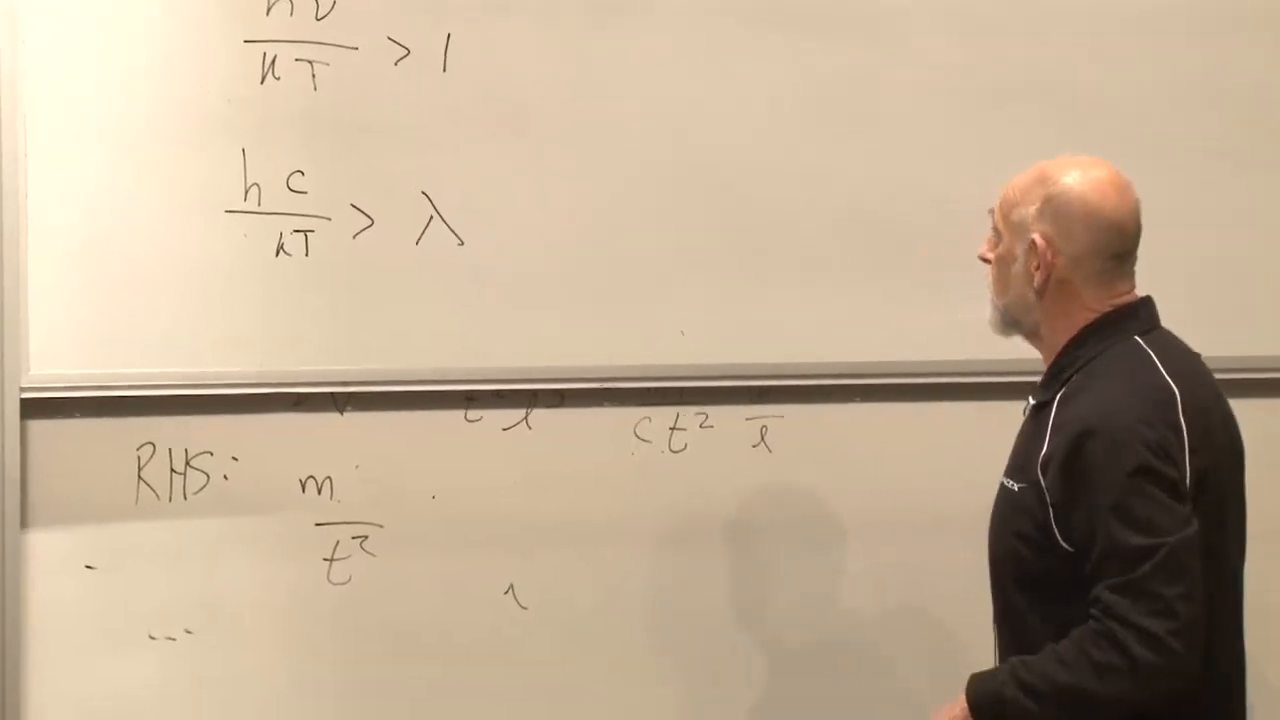
\includegraphics[width=0.82\textwidth]{lecture_07_figure_02.png}
\caption{Điểm chuyển tiếp nhiệt trên bảng. Biểu thức phía trên bị cắt cụt là \(h\nu/(kT)>1\), còn biểu thức phía dưới nhìn rõ là \(hc/(kT)>\lambda\). Những vết mờ còn sót lại ở phần bảng dưới không được dùng làm chứng cứ cho phương trình.}
\label{fig:c07-thermal-board}
\lectureframe{00:44:42.840}
\end{figure}

Dùng \(\nu=c/\lambda\), sự chuyển tiếp xác định một bước sóng nhiệt theo bậc độ lớn,
\begin{equation}
\boxed{\lambda_{\rm th}\sim\frac{hc}{k_BT}}.
\label{eq:c07-thermal-wavelength}
\end{equation}
Các bước sóng ngắn hơn nằm trong phần đuôi bị triệt giảm theo hàm mũ; phần lớn công suất được mang bởi các bước sóng cỡ này, sai khác bởi một hệ số số học phụ thuộc vào việc phổ được vẽ theo đơn vị tần số hay theo đơn vị bước sóng.

\begin{classroomqa}
\audiencequestion{Planck có thu được phổ này từ mô hình plasma electron--proton dùng ở đây không?}
\lecturerresponse{Không. Ông đã kết hợp thông tin phổ thực nghiệm với định luật dịch chuyển Wien, vốn đã cho thấy bước sóng cực đại biến thiên tỉ lệ nghịch với nhiệt độ. Quy luật tỉ lệ đó làm lộ ra một hằng số mới \(h\). Planck liên hệ kết quả này với các bộ dao động trong các vách vật chất, còn cách diễn giải lượng tử đầy đủ của trường bức xạ thì chỉ xuất hiện về sau. \lecturetimestamp{00:37:06--00:39:25}}
\end{classroomqa}

\begin{classroomqa}
\audiencequestion{Vì sao phép kiểm tra thứ nguyên dường như lại bỏ sót một lũy thừa của \(c\)?}
\lecturerresponse{Đại lượng lúc đầu được gọi là cường độ được định nghĩa là năng lượng trên một đơn vị thể tích trên một đơn vị tần số, trong khi công thức quen thuộc với \(2h\nu^3/c^2\) là độ chói phổ trên một đơn vị diện tích và góc khối. Mật độ năng lượng phổ mang \(c^{-3}\) và một hệ số góc, như trong phương trình~\eqref{eq:c07-planck}. Sự hiệu chỉnh này thay đổi quy ước chuẩn hóa, chứ không thay đổi tỉ số không thứ nguyên \(h\nu/(k_BT)\) hay bước sóng nhiệt. \lecturetimestamp{00:39:33--00:44:51}}
\end{classroomqa}

Ngoài hệ số chuẩn hóa, phổ Planck có một dạng phổ quát. Phương trình~\eqref{eq:c07-planck} có thể được viết thành
\begin{equation}
u_\nu(T)=T^3\,F\!\left(\frac{\nu}{T}\right),
\label{eq:c07-scaling-form}
\end{equation}
với các hằng số được hấp thụ vào \(F\). Tăng \(T\) sẽ co giãn lại trục tần số và cả chiều cao tổng thể; cùng một đường cong không thứ nguyên lại xuất hiện. Nếu diễn đạt theo bước sóng, tăng nhiệt độ sẽ nén phổ về phía các bước sóng ngắn hơn.

\begin{figure}[htbp]
\centering
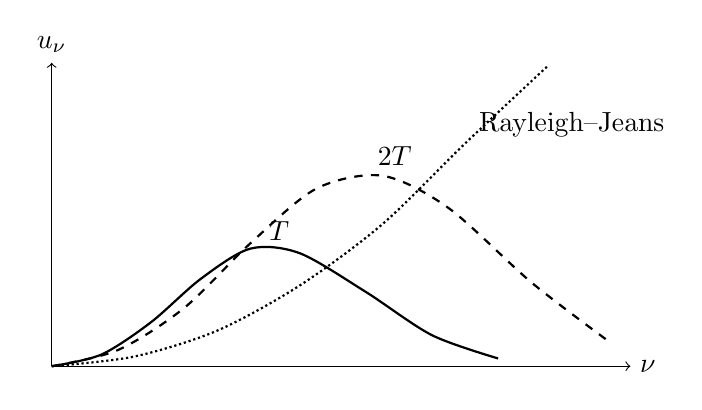
\begin{tikzpicture}[x=1.05cm,y=0.82cm]
\draw[->] (0,0)--(7.0,0) node[right] {\(\nu\)};
\draw[->] (0,0)--(0,4.7) node[above] {\(u_\nu\)};
\draw[densely dotted,thick] plot[smooth] coordinates
  {(0,0) (1,0.15) (2,0.55) (3,1.25) (4,2.20) (5,3.45) (6,4.65)};
\draw[thick] plot[smooth] coordinates
  {(0,0) (0.6,0.18) (1.2,0.68) (1.8,1.35) (2.4,1.82) (3.0,1.75) (3.8,1.15) (4.6,0.48) (5.4,0.12)};
\draw[thick,dashed] plot[smooth] coordinates
  {(0,0) (0.8,0.25) (1.6,0.90) (2.4,1.90) (3.2,2.75) (4.0,2.95) (4.8,2.45) (5.8,1.30) (6.7,0.42)};
\node[anchor=west] at (5.05,3.75) {Rayleigh--Jeans};
\node at (2.75,2.10) {\(T\)};
\node at (4.15,3.25) {\(2T\)};
\end{tikzpicture}
\caption{Phổ cổ điển tăng vô hạn, còn các phổ Planck thì đạt cực đại rồi giảm. Tăng nhiệt độ làm dịch tần số đặc trưng lên cao hơn và giữ nguyên hình dạng không thứ nguyên.}
\label{fig:c07-planck-redraw}
\end{figure}

Đại đa số photon trong vũ trụ hiện nay thuộc về phông vi ba và có bước sóng đặc trưng cỡ một milimét. Phương trình~\eqref{eq:c07-thermal-wavelength} liên hệ bước sóng đó với vài kelvin, ở đây theo thông lệ làm tròn thành \(3\,\mathrm{K}\). Chỉ riêng một bước sóng thì chỉ cho một liên hệ xấp xỉ. Bằng chứng mạnh hơn là các phép đo trên nhiều tần số vạch ra toàn bộ đường cong vật đen với độ chính xác rất cao.

\begin{classroomqa}
\audiencequestion{Một photon của phông vi ba chiếm bao nhiêu không gian?}
\lecturerresponse{Photon không có một kích thước cứng, ranh giới sắc nét mang tính phổ quát. Nó có thể được chuẩn bị như một gói sóng mà độ trải không gian phụ thuộc vào trạng thái, còn bước sóng của nó đặt ra thang cho dao động của nó. Đối với phông nhiệt, cả bước sóng đặc trưng lẫn một thang độ dài gói sóng tự nhiên đều cỡ một milimét, nhưng không nên nhầm một trong hai với bán kính của một vật thể cổ điển nhỏ. \lecturetimestamp{00:57:16--00:59:05}}
\end{classroomqa}

\section{Sự giãn nở giữ nguyên dạng phổ vật đen}

Xét một hộp nóng chứa hydro bị ion hóa và bức xạ ở trạng thái cân bằng. Khi hộp giãn nở, các thành phần bên trong thực hiện công, mật độ năng lượng giảm và nhiệt độ hạ xuống. Cuối cùng electron và proton liên kết bền thành các nguyên tử trung hòa. Sự hình thành nguyên tử được gọi là \emph{tái hợp}; sự mất đi của tán xạ photon--vật chất hữu hiệu được gọi là \emph{tách rời}. Hai quá trình này liên hệ chặt chẽ nhưng gọi tên những sự kiện vật lý khác nhau.

Sau khi tách rời, vật chất và bức xạ không còn có chung một nhiệt độ. Tuy vậy, phổ photon vẫn giữ dạng Planck. Mọi bước sóng truyền tự do đều bị kéo giãn bởi cùng một hệ số giãn nở,
\begin{equation}
\lambda\propto a,
\qquad
\nu\propto a^{-1}.
\end{equation}
Vì đường cong Planck phụ thuộc vào \(\nu/T\), dịch đỏ đồng đều này tương đương với việc gán cho bức xạ một nhiệt độ
\begin{equation}
\boxed{T_\gamma\propto a^{-1}.}
\label{eq:c07-temperature-scaling}
\end{equation}
Vì thế sự giãn nở giữ nguyên hình dạng ấy ngay cả khi không có các va chạm liên tục tái lập nó. Vật chất đi theo lịch sử nhiệt riêng của nó về sau.

Phông vi ba quan sát được vì thế là một phân bố cân bằng hóa thạch. Dạng vật đen của nó được xác lập khi sự tán xạ trên các điện tích tự do còn hữu hiệu, rồi sau đó được mang theo bởi dịch đỏ vũ trụ đồng đều. Ánh sao, tia gamma và các nguồn muộn hơn khác vẫn tồn tại, nhưng xét về số lượng chúng rất nhỏ bên cạnh quần thể photon di tích và có nguồn gốc vật lý thiên văn có thể nhận diện được.

\begin{classroomqa}
\audiencequestion{Làm sao bức xạ vẫn có thể giữ dạng vật đen sau khi nó không còn ở trạng thái cân bằng với vật chất nữa?}
\lecturerresponse{Va chạm là cần thiết để tạo ra phổ cân bằng, nhưng không cần để bảo toàn nó dưới sự giãn nở hoàn toàn đồng đều. Nhân mọi bước sóng với cùng một hệ số sẽ biến một phổ Planck thành một phổ khác có nhiệt độ thấp hơn. Các photon không còn chia sẻ nhiệt độ của vật chất, nhưng vẫn giữ một nhiệt độ vật đen của riêng mình.}
\end{classroomqa}

\section{Vì sao tái hợp xảy ra muộn đến vậy}

Bước sóng ngày nay và bước sóng tại thời điểm tách rời liên hệ với nhau bởi
\begin{equation}
\frac{\lambda_0}{\lambda_{\rm dec}}
=
\frac{a_0}{a_{\rm dec}}
=
\frac{T_{\rm dec}}{T_0}.
\label{eq:c07-decoupling-ratio}
\end{equation}
Sự tách rời không diễn ra tức thời theo nghĩa toán học, nhưng so với lịch sử tiếp theo thì nó đủ ngắn để ta có thể gán cho nó một hệ số tỉ lệ và một nhiệt độ đặc trưng. Ở đây \(T_0\) là nhiệt độ của CMB, không phải nhiệt độ động học của vật chất liên thiên hà.

Năng lượng ion hóa của trạng thái cơ bản của hydro là
\begin{equation}
\chi_H=13.6\,\mathrm{eV}.
\end{equation}
Một ước lượng đầu tiên sẽ đặt \(k_BT\sim\chi_H\), để một photon điển hình có thể ion hóa một nguyên tử. Ước lượng đó quá cao vì phổ nhiệt có một đuôi năng lượng cao và vũ trụ chứa một số lượng photon khổng lồ.

\begin{figure}[htbp]
\centering
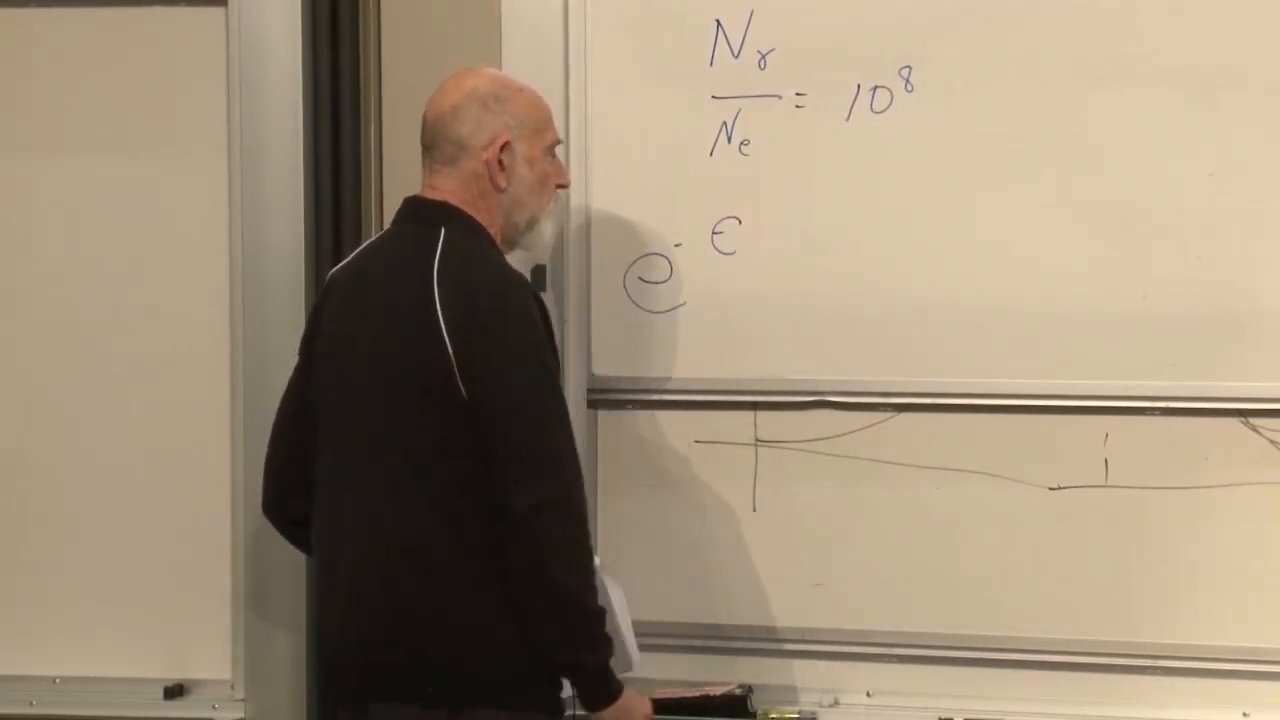
\includegraphics[width=0.82\textwidth]{lecture_07_figure_03.png}
\caption{Trên bảng xuất hiện tỉ số độ phong phú quan sát được \(N_\gamma/N_e=10^8\) và ký hiệu năng lượng photon \(\epsilon\). Chỉ thấy phần đầu của hàm mũ; thừa số Boltzmann hoàn chỉnh được suy ra từ phần diễn giải bằng lời.}
\label{fig:c07-boltzmann-board}
\lectureframe{01:06:10.631}
\end{figure}

Tỉ số độ phong phú làm tròn được dùng ở đây là
\begin{equation}
\frac{N_\gamma}{N_e}\sim10^8.
\label{eq:c07-photon-electron-ratio}
\end{equation}
Nó được suy ra bằng cách so sánh mật độ photon CMB đo được với kiểm kê vật chất thường. Với năng lượng photon \(\epsilon\), phần đuôi năng lượng cao có dạng Boltzmann
\begin{equation}
P(\epsilon)\propto e^{-\epsilon/(k_BT)}.
\end{equation}
Vì vậy số photon ion hóa sẵn có trên mỗi nguyên tử được ước lượng bởi
\begin{equation}
10^8 e^{-\chi_H/(k_BT)}.
\end{equation}
Sự ion hóa vẫn còn hiệu quả cho đến khi đại lượng này giảm xuống cỡ đơn vị.

Lấy lôgarit cho
\begin{equation}
\frac{\chi_H}{k_BT}
\sim
\ln 10^8
\simeq18.4,
\end{equation}
hay, ở độ chính xác nhắm tới ở đây,
\begin{equation}
k_BT\sim\frac{\chi_H}{20}.
\label{eq:c07-tail-estimate}
\end{equation}
Photon đặc trưng có thể nằm thấp hơn ngưỡng khá xa, vì đối với mỗi nguyên tử chỉ cần một photon ion hóa từ phần đuôi là đủ.

\begin{classroomqa}
\audiencequestion{Ước lượng từ phần đuôi đếm các photon đúng tại ngưỡng hay tất cả các photon ở phía trên nó?}
\lecturerresponse{Nó đếm các photon ở ngưỡng và phía trên ngưỡng. Vì phần đuôi suy giảm theo hàm mũ, phần lớn tích phân đó đến từ các năng lượng gần \(\chi_H\), nên ước lượng mũ đơn giản nắm được đúng bậc độ lớn liên quan. \lecturetimestamp{01:08:39--01:08:54}}
\end{classroomqa}

\begin{classroomqa}
\audiencequestion{Tỉ số \(N_\gamma/N_e\) tại thời điểm tách rời cũng vào khoảng \(10^8\) hay sao?}
\lecturerresponse{Theo gần đúng được dùng ở đây thì có. Từ thời điểm tách rời trở lui về các thời kỳ nóng hơn đáng kể, sự giãn nở làm loãng cả hai quần thể theo cùng một hệ số thể tích và không tạo ra hay phá hủy đủ của một trong hai loại để làm thay đổi tỉ số của chúng. Ở những nhiệt độ còn cao hơn nữa, các phản ứng tạo cặp đòi hỏi phải hạch toán lại. \lecturetimestamp{01:08:54--01:09:57}}
\end{classroomqa}

\begin{classroomqa}
\audiencequestion{Các photon do sao phát ra có đóng góp đáng kể vào phép đếm này không?}
\lecturerresponse{Không. Các ngôi sao vào thời tái hợp còn chưa tồn tại, và ngay cả ngày nay các photon của chúng cũng chỉ là một phần cực nhỏ của quần thể CMB. Tỉ số trong phương trình~\eqref{eq:c07-photon-electron-ratio} liên quan đến các photon nhiệt di tích. \lecturetimestamp{01:11:44--01:12:39}}
\end{classroomqa}

\begin{classroomqa}
\audiencequestion{Khi electron tái hợp với proton, các photon phát ra có để lại một đặc trưng hydro sắc nét trong phổ vật đen không?}
\lecturerresponse{Chừng nào tán xạ và hấp thụ vẫn còn nhanh so với sự giãn nở, bức xạ vẫn liên tục được tái xử lý và duy trì gần cân bằng nhiệt. Một sự đóng băng đủ đột ngột có thể bảo toàn một méo dạng, nhưng sự tái hợp chậm, gần cân bằng ngăn không cho một vạch cô lập lớn thay thế dạng vật đen. \lecturetimestamp{01:12:42--01:14:07}}
\end{classroomqa}

Ước lượng thu được trên lớp là \(T_{\rm dec}\sim4\times10^3\,\mathrm{K}\). Việc chuyển đổi trực tiếp \(\chi_H/20\) cho ra một giá trị hơi cao hơn, từ đó gợi ý rằng mẫu số hiệu dụng có thể gần \(40\) hơn. Đây không phải là mâu thuẫn; nó cho thấy sự thô sơ của việc thay thế cân bằng ion hóa đầy đủ bằng một phép đếm đơn lẻ ở phần đuôi. Một xử lý cân bằng có kiểm soát dùng hệ thức Saha,
\begin{equation}
\frac{x_e^2}{1-x_e}
=
\frac{1}{n_H}
\left(\frac{m_e k_BT}{2\pi\hbar^2}\right)^{3/2}
e^{-\chi_H/(k_BT)},
\label{eq:c07-saha}
\end{equation}
rồi tiếp theo là động học tái hợp ngoài cân bằng. Lập luận thô này có giá trị vì nó chỉ ra vật lý chi phối: tỉ số baryon trên photon rất nhỏ trì hoãn thời điểm các nguyên tử trung hòa có thể tồn tại bền vững tới một nhiệt độ thấp hơn nhiều so với \(\chi_H/k_B\).

\section{Dịch đỏ tới mặt tán xạ cuối cùng}

Với \(T_0\simeq3\,\mathrm{K}\) và \(T_{\rm dec}\sim4\times10^3\,\mathrm{K}\), phương trình~\eqref{eq:c07-decoupling-ratio} cho
\begin{equation}
\boxed{
\frac{a_0}{a_{\rm dec}}
\sim
\frac{T_{\rm dec}}{T_0}
\sim10^3
}.
\label{eq:c07-decoupling-expansion}
\end{equation}
Tương đương, dịch đỏ của tán xạ cuối cùng vào cỡ \(10^3\). Trước thời kỳ này plasma ion hóa là môi trường mờ đục; sau đó, các photon truyền gần như tự do.

Sự kiện nhiệt này chỉ xảy ra vài trăm nghìn năm sau khi bắt đầu sự giãn nở nóng, trong phần trao đổi được nêu theo thông lệ là xấp xỉ \(380{,}000\) năm. Khoảng thời gian ấy là rất nhỏ so với tuổi vũ trụ tiếp theo. Kể từ khi tách rời, các độ dài đã tăng khoảng \(10^3\) và các phần tử thể tích đồng chuyển đã tăng khoảng \(10^9\).

Tách rời là một mốc nhiệt, chứ không phải sự kiện duy nhất trong lịch sử xen giữa. Sự hình thành thiên hà, sự hình thành sao và sự hình thành lỗ đen đều xảy ra muộn hơn, nhưng ở đây chúng được gác sang một bên để có thể lần ngược các mốc nhiệt một cách rõ ràng.

Nhìn ra xa là nhìn ngược về quá khứ. Các lớp vỏ gần cho thấy những thời kỳ gần đây; các lớp vỏ xa hơn cho thấy những thời kỳ sớm hơn. Nón ánh sáng quá khứ của chúng ta cuối cùng gặp thời kỳ tái hợp, và giao của nó với thời kỳ ấy là mặt tán xạ cuối cùng. Bức xạ điện từ sớm hơn đã nhiều lần bị các điện tích tự do tán xạ và không thể truyền thẳng tới chúng ta.

\begin{figure}[htbp]
\centering
\begin{coursefitfigure}
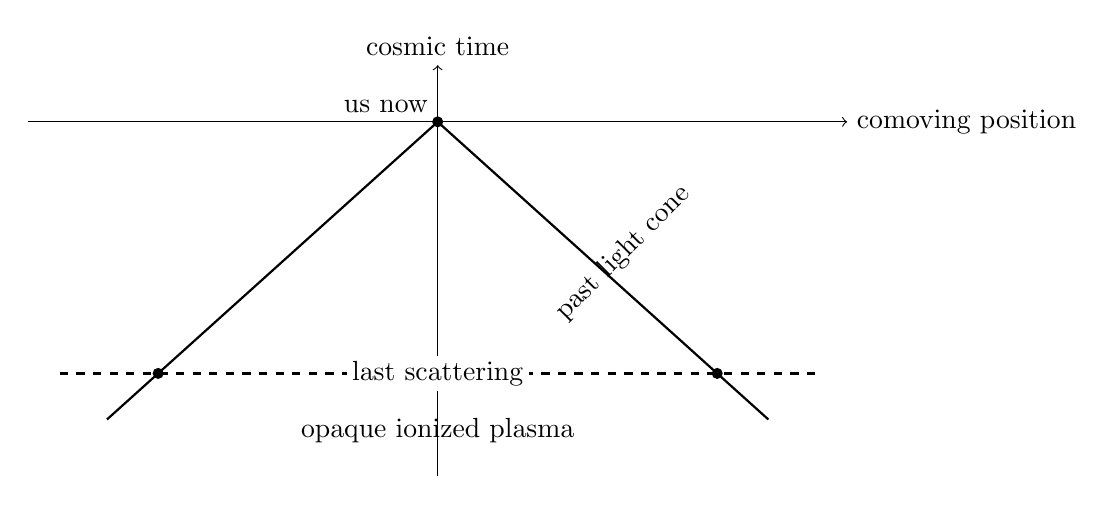
\begin{tikzpicture}[x=1.0cm,y=0.9cm]
\draw[->] (0,0)--(0,5.8) node[above] {cosmic time};
\draw[->] (-5.2,5.0)--(5.2,5.0) node[right] {comoving position};
\draw[thick] (0,5.0)--(-4.2,0.8);
\draw[thick] (0,5.0)--(4.2,0.8);
\draw[thick,dashed] (-4.8,1.45)--(4.8,1.45);
\fill (0,5.0) circle (2pt) node[above left] {us now};
\fill (-3.55,1.45) circle (2pt);
\fill (3.55,1.45) circle (2pt);
\node[fill=white,inner sep=2pt] at (0,1.45) {last scattering};
\node at (0,0.65) {opaque ionized plasma};
\node[rotate=45] at (2.35,3.15) {past light cone};
\end{tikzpicture}
\end{coursefitfigure}
\caption{Quan sát điện từ chỉ lần ngược dọc theo nón ánh sáng quá khứ tới mặt tán xạ cuối cùng. Các photon sớm hơn đã bị plasma ion hóa tán xạ lặp đi lặp lại.}
\label{fig:c07-last-scattering}
\end{figure}

\begin{classroomqa}
\audiencequestion{Việc tách rời có chấm dứt mọi khả năng quan sát các thời kỳ sớm hơn không?}
\lecturerresponse{Nó chấm dứt quan sát điện từ trực tiếp vì plasma mờ đục đối với photon. Những sứ giả tương tác yếu hơn có thể thoát ra sớm hơn: về nguyên tắc, neutrino di tích thăm dò được một lớp sâu hơn, và bức xạ hấp dẫn có thể mang thông tin từ còn sớm hơn nữa. Vì thế, phần lớn hiểu biết của chúng ta về các thời kỳ trước mặt tán xạ cuối cùng là gián tiếp, nhưng không tùy tiện. \lecturetimestamp{01:32:27--01:36:31}}
\end{classroomqa}

\begin{classroomqa}
\audiencequestion{Giá trị tuyệt đối của \(a\) lúc ban đầu là bao nhiêu, và vũ trụ có nhất thiết là một vật thể nhỏ hữu hạn không?}
\lecturerresponse{Trong không gian phẳng, chỉ các tỉ số của thừa số tỉ lệ mới có ý nghĩa bất biến; việc chuẩn hóa \(a\) là tùy ý. Một lát cắt không gian có độ cong âm cũng có thể là vô hạn. Một vũ trụ đóng \(k=+1\) có bán kính cong hữu hạn, nhưng quan sát vẫn xác định các tỉ số giãn nở chứ không phải một kích thước nguyên thủy đã biết. Bản thân Vụ Nổ Lớn nóng không phải là phát biểu rằng toàn bộ không gian từng là một quả cầu nhỏ. \lecturetimestamp{01:30:05--01:32:22}}
\end{classroomqa}

\begin{classroomqa}
\audiencequestion{Vì CMB cổ hơn các thiên hà, việc quan sát nó có cho ta biết liệu ngày nay có các thiên hà ở ngoài vùng quan sát được của ta hay không?}
\lecturerresponse{Không. CMB cho ta thấy một vùng xa xôi như nó đã ở thời tách ghép, chứ không phải như hiện nay. Ánh sáng từ các thiên hà ngày nay ở những khoảng cách đủ lớn vẫn chưa có thời gian đến được chỗ ta. Điều ủng hộ khả năng các quần thể thiên hà tiếp tục tồn tại bên ngoài chân trời của ta là tính đồng nhất trên quy mô lớn đã quan sát được và sự vắng mặt của một rìa nhìn thấy được, chứ không phải một cái nhìn trực tiếp do CMB cung cấp. \lecturetimestamp{01:59:01--02:00:58}}
\end{classroomqa}

Dòng thời gian thu được đi ngược từ hiện tại, qua sự hình thành thiên hà và sự tách ghép, đến thời điểm vật chất--bức xạ bằng nhau. Lùi sớm hơn nữa, thừa số tỉ lệ co lại đồng nghĩa với nhiệt độ tăng lên và sự xuất hiện của các loài hạt mới.

\section{Cân bằng vật chất--bức xạ}

Đi ngược về quá khứ qua mốc tách ghép, một cột mốc khác xuất hiện. Vật chất phi tương đối tính và bức xạ bị pha loãng theo những cách khác nhau:
\begin{equation}
\rho_m\propto a^{-3},
\qquad
\rho_r\propto a^{-4},
\qquad
\frac{\rho_m}{\rho_r}\propto a.
\label{eq:c07-equality-scaling}
\end{equation}
Vật chất chi phối ở thời muộn, nhưng ở \(a\) đủ nhỏ thì bức xạ tất yếu chi phối. Theo đó, định luật giãn nở chuyển từ dạng của kỷ nguyên vật chất \(a\propto t^{2/3}\) sang dạng của kỷ nguyên bức xạ \(a\propto t^{1/2}\).

Một ước lượng cố ý thô bắt đầu từ \(10^8\) photon trên mỗi proton, năng lượng photon CMB đặc trưng \(10^{-4}\,\mathrm{eV}\), và năng lượng nghỉ của proton \(10^9\,\mathrm{eV}\). Nếu bỏ qua vật chất tối thì ta có
\begin{equation}
\left(\frac{\rho_m}{\rho_r}\right)_0
\sim
\frac{10^9}{10^8\,10^{-4}}
\sim10^5.
\end{equation}
Lập luận sau đó tự điều chỉnh: vật chất tối đóng góp khối lượng lớn hơn đáng kể so với các baryon phát sáng, nâng ước lượng làm tròn lên \(10^6\). Trong phép tính này, phương trình~\eqref{eq:c07-equality-scaling} đặt thời điểm bằng nhau tại
\begin{equation}
\frac{a_{\rm eq}}{a_0}\sim10^{-6},
\qquad
\frac{T_{\rm eq}}{T_0}\sim10^6.
\label{eq:c07-equality-estimate}
\end{equation}
Đây là các ước lượng trên lớp nhằm xác định thang độ, không phải một phép khớp tham số vũ trụ học chính xác. Mục đích của chúng là chỉ ra cách các lũy thừa khác nhau của \(a\) định vị các kỷ nguyên nhiệt kế tiếp nhau.

Kỷ nguyên bức xạ chi phối nằm phía sau bức tường tán xạ cuối cùng điện từ, nhưng sự tồn tại của nó suy ra từ các mật độ thời muộn đã đo được và các luật tỉ lệ đã biết. Đi lên nhiệt độ cao hơn nữa cuối cùng sẽ làm mất hiệu lực giả thiết rằng số proton, electron và photon được cố định riêng rẽ, vì các va chạm đủ năng lượng bắt đầu tạo ra các cặp hạt--phản hạt có khối lượng.

\begin{classroomqa}
\audiencequestion{Phát biểu rằng số photon và số proton được bảo toàn có bao gồm ánh sáng sao và các nhiệt độ cao tùy ý không?}
\lecturerresponse{Không. Nó áp dụng cho quần thể CMB tàn dư trong giai đoạn mà các phản ứng làm thay đổi số hạt không còn hiệu quả. Ánh sáng sao được tạo ra về sau và không đáng kể trong tổng số photon. Ở nhiệt độ đủ cao, sự tạo cặp làm thay đổi thành phần hạt và sự bảo toàn số riêng rẽ không còn đúng. Bản thân sự tái hợp nhiều nhất chỉ thêm xấp xỉ 1 photon cho mỗi electron, tức chỉ bằng một phần trong \(10^8\) của quần thể CMB sẵn có. \lecturetimestamp{01:26:24--01:27:40}}
\end{classroomqa}

\section{Sự tạo cặp và súp hạt gần đối xứng}

Ở nhiệt độ cỡ
\begin{equation}
T\sim10^{10}\,\mathrm{K},
\qquad
\frac{a_0}{a}\sim10^{14},
\end{equation}
năng lượng photon đặc trưng vào khoảng một mega-electron-volt, so sánh được với thang năng lượng nghỉ cần để tạo ra một cặp electron--positron. Khi đó hai photon có thể phản ứng theo
\begin{equation}
\gamma+\gamma
\longleftrightarrow
e^-+e^+.
\label{eq:c07-pair-reaction}
\end{equation}
Ngưỡng chính xác phụ thuộc vào động học va chạm, nhưng năng lượng nghỉ của electron, \(m_ec^2\), đặt ra thang liên quan.

Sự tạo cặp và sự hủy cặp nhanh chóng cân bằng lẫn nhau. Nếu có quá ít cặp, các va chạm photon sẽ bổ sung chúng; nếu có quá nhiều, sự hủy cặp trả năng lượng của chúng về cho photon. Vì vậy, độ phong phú của photon, electron và positron do nhiệt độ quyết định và trong plasma tương đối tính đều cùng bậc độ lớn. Chúng không còn giữ một ký ức đơn giản về số lượng về sau của mình.

\begin{classroomqa}
\audiencequestion{Làm sao plasma đầy các cặp này vẫn có thể trung hòa điện khi đã có sẵn các electron cần để cân bằng proton?}
\lecturerresponse{Mỗi phản ứng tạo ra một điện tích âm và một điện tích dương, nên các cặp không thêm điện tích thuần. Chúng là một quần thể khổng lồ gần đối xứng chồng lên một phần dư electron rất nhỏ. Các electron riêng lẻ là không thể phân biệt; chỉ có hiệu \(N_{e^-}-N_{e^+}\) còn ghi nhớ điện tích cần để cân bằng proton. \lecturetimestamp{01:42:31--01:43:14}}
\end{classroomqa}

Các phản ứng tạo-hủy cặp làm thay đổi tổng nhưng bảo toàn hiệu:
\begin{equation}
N_{e^-}+N_{e^+}\quad\hbox{changes},
\qquad
N_{e^-}-N_{e^+}=\hbox{constant}.
\label{eq:c07-pair-invariants}
\end{equation}
Trong súp hạt nóng, \(N_{e^-}+N_{e^+}\) cùng bậc với \(N_\gamma\), còn phần dư còn lại cùng bậc với số proton nhỏ hơn rất nhiều. Do đó tỉ số làm tròn là
\begin{equation}
\boxed{
\frac{N_{e^-}-N_{e^+}}
{N_{e^-}+N_{e^+}}
\sim10^{-8}
}.
\label{eq:c07-asymmetry}
\end{equation}
Có xấp xỉ 1 electron dư trên mỗi \(10^8\) cặp electron--positron.

Điều này đảo ngược câu hỏi ban đầu. Sự thật nổi bật không chỉ đơn giản là photon rất nhiều. Ở nhiệt độ cao, photon và các cặp tự nhiên có độ phong phú tương đương. Điều khó hiểu là vì sao quần thể hạt âm và hạt dương lại khác nhau chút nào, và vì sao độ chênh lệch tương đối của chúng lại rất nhỏ thay vì chính xác bằng không hoặc cỡ đơn vị. Một trạng thái ban đầu đối xứng và sự tạo cặp đối xứng sẽ không tạo ra phần dư thừa nào. Nguồn gốc vi mô của sự bất đối xứng khác không ấy là vấn đề được chuyển sang giai đoạn tiếp theo của phần thảo luận.

Ở các nhiệt độ cao hơn thêm 2 hoặc 3 bậc độ lớn, cấu trúc proton không thể bỏ qua nữa. Các va chạm tạo ra quark và phản quark, trong khi proton tan thành các thành phần cấu tạo của chúng; photon, lepton, quark, phản quark, gluon, và mọi loài hạt tối đủ nhẹ cùng tạo thành một plasma nóng hơn. Ở đó năng lượng chân không là không đáng kể về mặt động lực học vì mật độ bức xạ tăng theo \(a^{-4}\).

Phần dư quark tương ứng gắn với phần dư electron bởi điều kiện trung hòa điện tổng thể. Ba quark hóa trị tạo thành một baryon, nên việc hạch toán khác đi do các hệ số quy ước, nhưng vật chất baryon còn sót lại và các electron còn sót lại không phải là những độ mất cân bằng điện tích độc lập. Sự nhỏ bé chung của chúng là di tích của vũ trụ sơ khai.

Hãy theo plasma electron--positron tiến về phía trước một lần nữa. Khi nhiệt độ hạ xuống dưới thang tạo cặp, sự hủy cặp tiếp tục trong khi phản ứng ngược trở nên hiếm. Gần như mọi electron đều gặp một positron, năng lượng của cặp trở thành bức xạ, và chỉ còn lại quần thể electron không có cặp rất nhỏ. Vật chất quanh ta chính là phần mất cân bằng còn dư này, không phải một mẫu đại diện của quần thể cặp từng khổng lồ ấy.

\begin{classroomqa}
\audiencequestion{Các proton đang làm gì trong thời kỳ hủy cặp electron--positron?}
\lecturerresponse{Ở giai đoạn đó, nhiệt độ đủ cao để tạo các cặp electron nhưng vẫn chưa đủ cao để tạo dồi dào các cặp proton--phản proton hoặc hòa tan proton thành quark. Vì vậy quần thể proton ít nhưng vẫn tồn tại, và điều kiện trung hòa đòi hỏi \(N_{e^-}-N_{e^+}\simeq N_p\). \lecturetimestamp{01:55:35--01:56:53}}
\end{classroomqa}

Vũ trụ khả kiến dường như ở khắp nơi đều có cùng một dấu của phần dư vật chất. Bằng chứng trên lớp được nêu ra là sự vắng mặt của các phản hạt nhân trong tia vũ trụ: các va chạm thứ cấp có thể đôi khi tạo ra phản proton, nhưng một phản thiên hà sẽ được kỳ vọng cung cấp các phản hạt nhân phức tạp. Đây là một lập luận quan sát ở mức bài giảng, không phải là tuyên bố rằng các vùng vượt quá chân trời quan sát đã được khảo sát.

\begin{classroomqa}
\audiencequestion{Liệu phần dư vật chất được quan sát có thể chỉ là một thăng giáng cục bộ, với các vùng phản vật chất nằm ngoài phần mà ta có thể thấy hay không?}
\lecturerresponse{Cùng một dấu trên toàn bộ thể tích quan sát được khổng lồ là quá nhất quán để có thể là một thăng giáng ngẫu nhiên. Nó đòi hỏi một lời giải thích động lực học. Tuy nhiên, bên ngoài vùng quan sát được thì không có bằng chứng trực tiếp; không thể loại trừ một chuyển tiếp sang một miền khác chỉ bằng cách nhìn xa hơn quãng mà ánh sáng đã kịp tới chỗ ta. \lecturetimestamp{01:56:57--01:58:47}}
\end{classroomqa}

\begin{classroomqa}
\audiencequestion{Liệu cách giải thích vật chất--phản vật chất đã là một lý thuyết định lượng chính xác hay chưa, và sự hợp nhất các lực có xảy ra ở nhiệt độ này không?}
\lecturerresponse{Có một lý thuyết định tính về cách một bất đối xứng nhỏ có thể nảy sinh, nhưng giá trị làm tròn \(10^{-8}\) ở đây không được suy ra từ một mô hình vi mô duy nhất. Sự hợp nhất các lực thuộc về các nhiệt độ cao hơn nhiều so với kỷ nguyên cặp electron. Cả hai câu hỏi đều đòi hỏi vật lý vượt ra ngoài các mốc nhiệt hiện đang xét. \lecturetimestamp{01:51:36--01:52:24}}
\end{classroomqa}

\section{Những điều cần ghi nhớ cho phần sau}

Lịch sử nhiệt được chi phối bởi các tốc độ và các ngưỡng. Sự tán xạ nhanh thiết lập một nhiệt độ chung; sự hình thành các nguyên tử trung hòa loại bỏ các hạt tán xạ; rồi sự giãn nở đồng đều làm dịch đỏ một phổ Planck đã đông cứng mà không phá hủy hình dạng của nó. Vì thế, CMB vừa là nhiệt kế của bức xạ vừa là một bề mặt khả kiến đánh dấu sự chấm dứt của khả năng tiếp cận điện từ trực tiếp đối với plasma tồn tại trước đó.

Sự dư thừa photon khiến quá trình tái hợp trở thành một bài toán của phần đuôi chứ không phải một bài toán của năng lượng trung bình. Mốc \(T_{\rm dec}/T_0\sim10^3\) xác định thời điểm tán xạ cuối cùng, trong khi các quy luật pha loãng không như nhau của vật chất và bức xạ xác định một thời kỳ cân bằng vật chất-bức xạ sớm hơn. Ở nhiệt độ còn cao hơn nữa, sự tạo cặp xóa mất thông tin về tổng số electron và positron nhưng vẫn giữ lại độ chênh rất nhỏ giữa chúng. Sự bất đối xứng còn dư đó, được phản chiếu trong phần baryon, là dữ kiện ban đầu chưa được giải thích mà cuộc khảo sát tiếp theo phải đối mặt.